\documentclass[11pt, english]{uspatent}
%\usepackage{fullpage}

% includes the figures information
\include{Drawings}
\usepackage{sidecap}
\usepackage{graphicx}
\graphicspath{ {images/} }

\begin{document}
\section*{Serial Number:}
X7BH76901J
\setAssigneeName{University of California, Santa Cruz}
\setAssigneeAddress{1156 High Street}
\setAssigneeCity{Santa Cruz}
\setAssigneePhone{(831) 459-0111}
\setDocketNumber{US26789101A}

\setDocumentVersion{0.0}
\setPrintingModeApplication

\title{Electrically Heated Boot Sock Made With Silicone Rubber}
\inventor{Shreya Reddy}
\date{}
\maketitle

\patentSection{Abstract}
\footnote{Taken idea from half bakery and google patent.}This invention is designed to protect people from extreme cold weathers. The model relates to a silicone rubber electrically heated boot sock and a sac to hold the battery. The boots are designed to be water proof and have the ability to adjust the temperature.The sac is built of a foldable sheet to store the battery. The boots comprises an overshoe to contour the foot from the ankle to toes. Also the pocket is formed to define a path which extends along one side through which a conductor gets in contact to heat the boots.

\patentSection{Prior Art}

\patentParagraph US07931025. Filing Date: 1992-08-17. Inflatable sole lining for shoes and boots
\patentParagraph US08453754. Filing Date: 1997-05-19. Interference suppressing cable boot assembly
\patentParagraph US5797862A. Filling Date: 1998-08-25. Medical boot for patient with diabetic foot
\patentParagraph  US07054189. Filling Date: 1987-05-26. Shoe with foot warmer including an electrical generator
\patentParagraph CA 582452. Filling Date: 1988-11-07. Heated and cooled boot and suit with forced air circulation

\patentSection{Representative Drawing}

\begin{figure}[h]
	\centering
	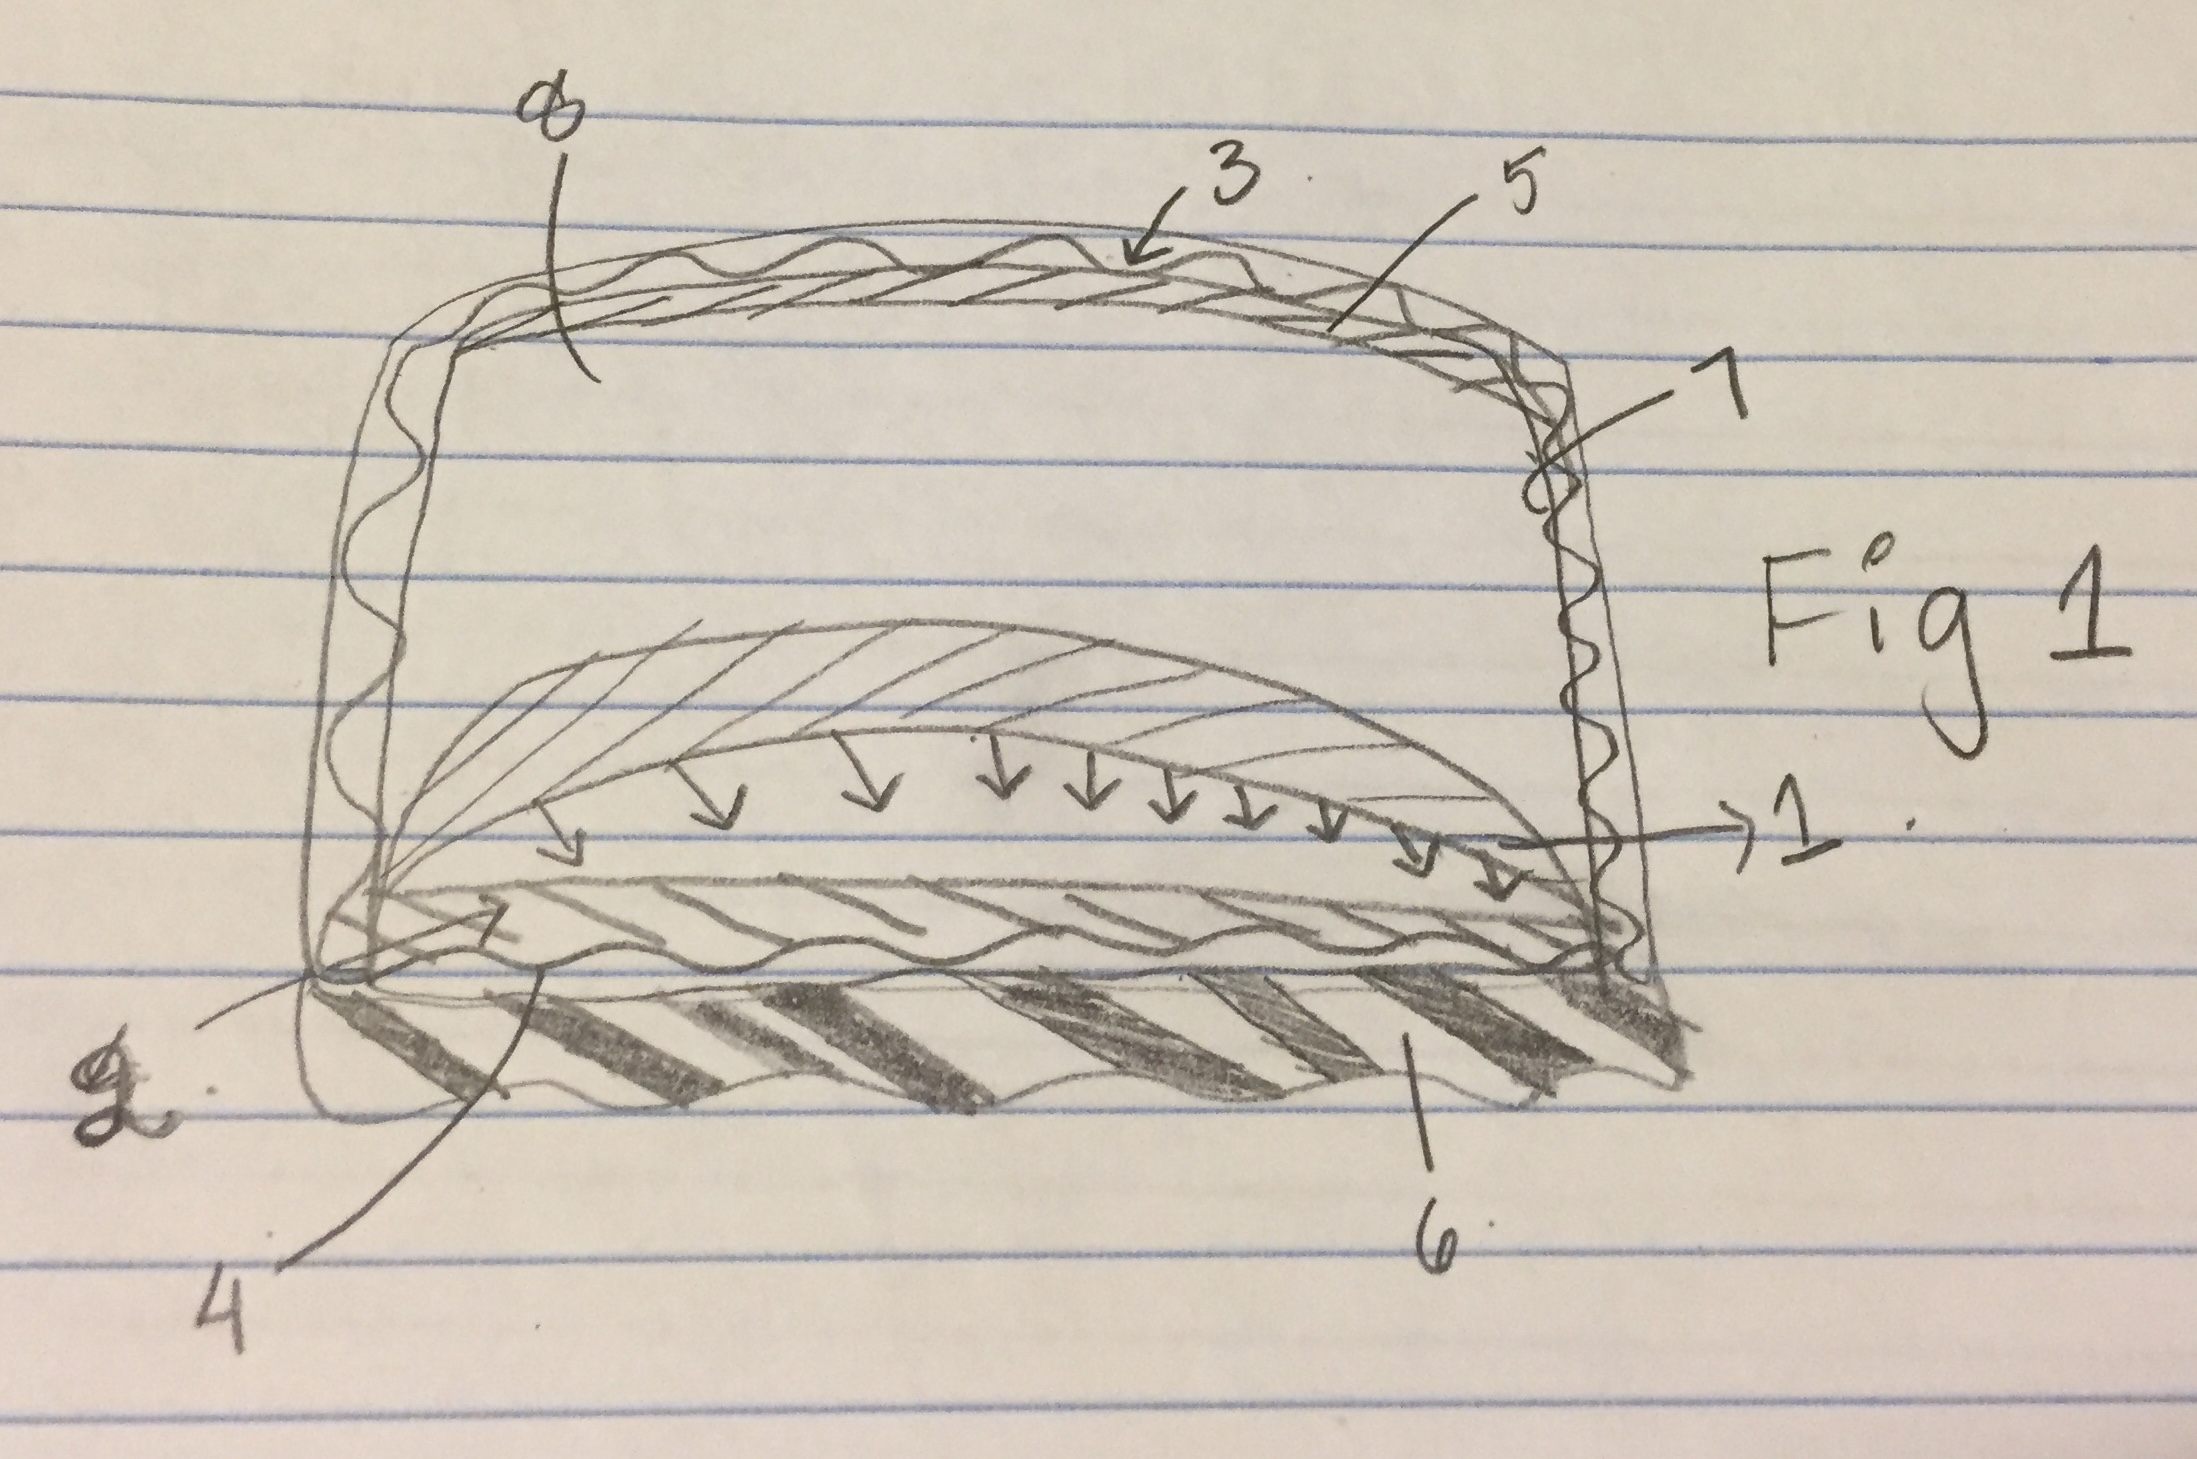
\includegraphics[width=8cm, height=8cm]{Fig1.jpg} 
	\label{fig:fig1}
\end{figure}

\begin{figure}[h]
	\centering
	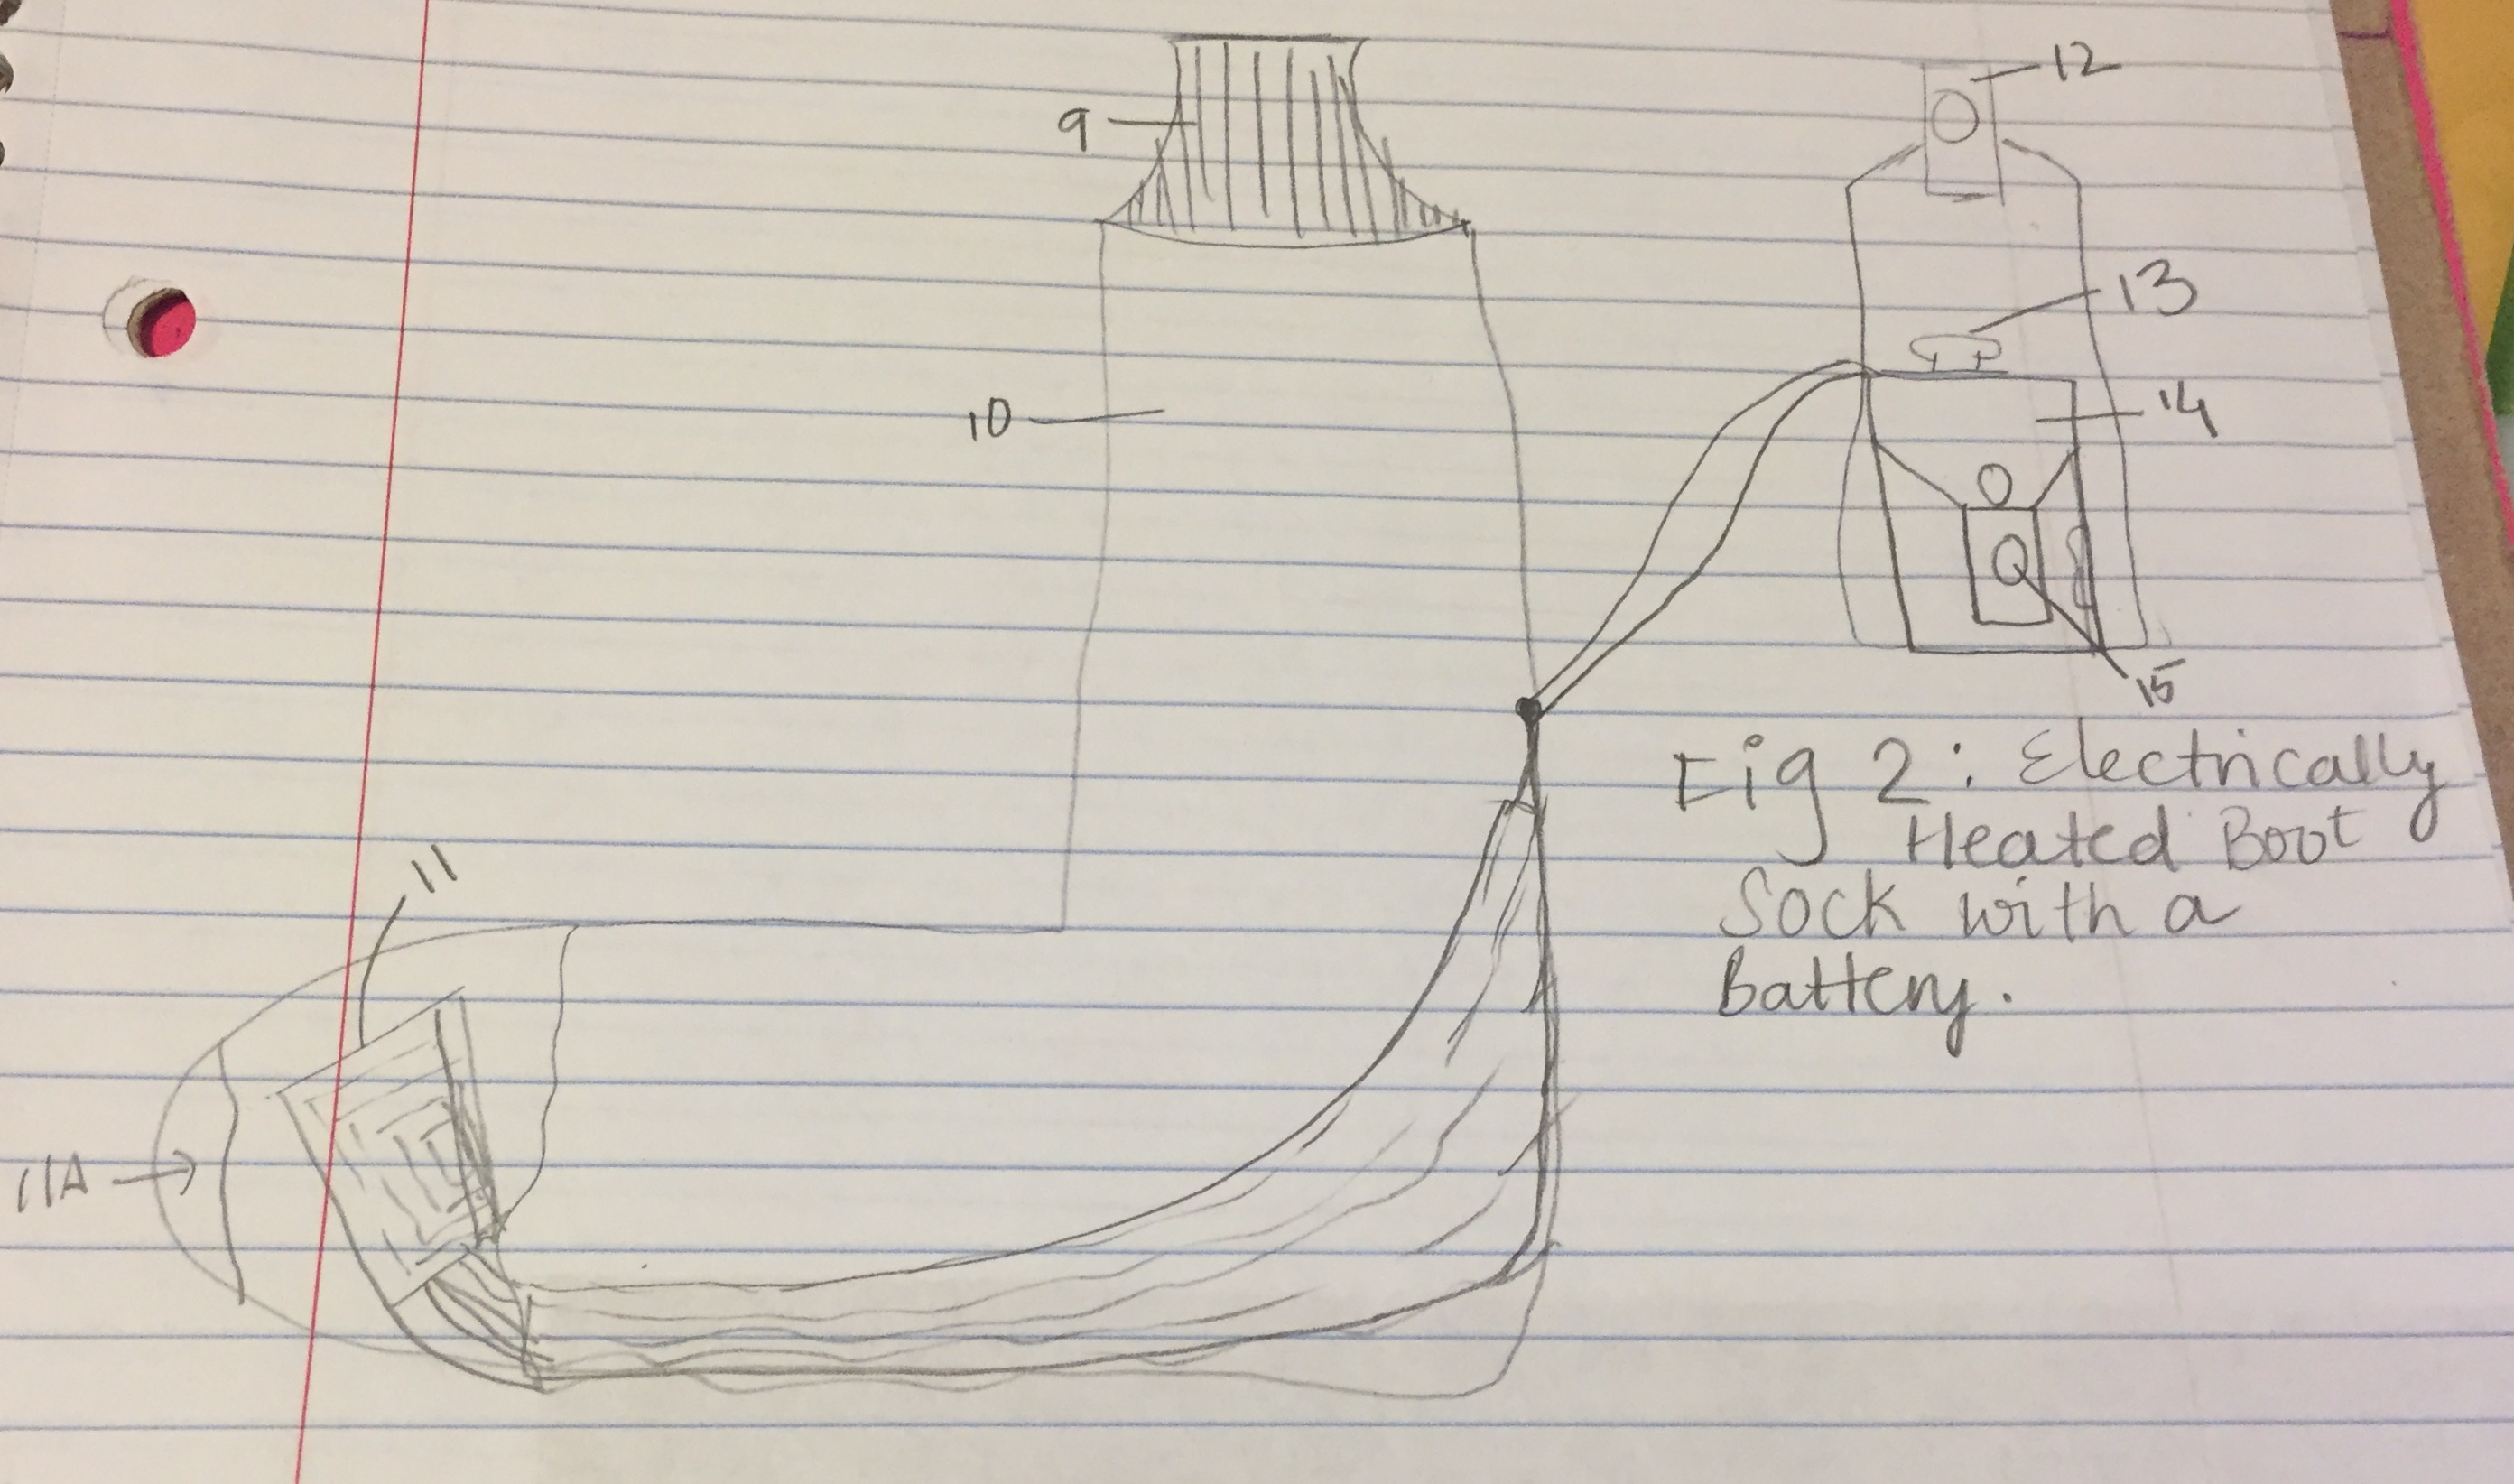
\includegraphics[width=8cm, height=8cm]{Fig2.jpg} 
	\label{fig:fig2}
\end{figure}


\patentSection{Background of the Invention}

\patentParagraph The invention of the boots relates to the construction and in particular for people living in cold cities. These boots are also perfect for people who go for hunting during the winter season or doing any activity(water related or snow activities) during the winter.
\patentParagraph Living in a place where it is cold throughout the year and trying to insulate your your body is very important. Especially the feet since they have a tendency to become cold and sometimes even frostbitten.
\patentParagraph So the electrically heated boots which are made of silicone rubber are provided to protect the feet from the cold. It comes with a temperature control wher the person can control how heated they want the boots.

\patentSection{Summary of the Invention}

\patentParagraph The invention of the electrically heated boots is designed in such a way that generates heat to the toes. The boots have a low voltage battery pouch connected to the panel and a temperature controller to control how much heat the person wants to supply to the boots.

\patentSection{Brief description of the drawings}

\patentParagraph Fig 1. is the top view of the boot sock that is constructed according to the invention.
\patentParagraph Fig 2. it represents the side elevation of the battery and temperature controller. It also represents a perspctive view of the heated sock when worn with winter clothing.

\patentSection{Detailed description of the invention}

\patentParagraph Referring to the drawings, the electrically heated boot which are numbered 1-15 shows how the boot is designed with the above mentioned features. This includes an overshoe extending from the wearer's ankle to toes. The sole member has the general outline of the wearer's foot.
\patentParagraph Formed between the shoes and the insulated web is a pocket portion of the sock where the low voltage battery is inserted.The heat produced by the boot can be controlled by the temperature controller. 
\patentParagraph Therefore, the boot is adapted to be heated during the cold weather by the warmer. And is used only during the winter seasons.

\patentClaimsStart
\beginClaim{Claim1}
A battery operated on low voltage electric boot sock comprises:
\begin{itemize}[label={}]
\item a foot portion having a toe portion and a heel portion and a connected lef portion. This is connected to the low voltage battery.
\item a conductir receiving means extending along one side of the sac for receiving the conductor connecting said one conatct.
\end{itemize}

\beginClaim{Claim2}
A hook connected to the sac, the hook that haves a tongue portion spaced from the sac, said tongue portion being adapted to frictionally engage the boot of the wearer.

\patentClaimsEnd

\end{document}